\pdfoutput=1
\documentclass{article}


% alptex + small aesthetic tweaks + some extra math defs
%\RequirePackage[l2tabu, orthodox]{nag}

% FONTS
\usepackage[utf8]{inputenc} % allow utf-8 input
\usepackage[T1]{fontenc}    % use 8-bit T1 fonts

% Replace default Latin Modern typewriter with its proportional counterpart
% http://www.tug.dk/FontCatalogue/lmoderntypewriterprop/
\renewcommand*\ttdefault{lmvtt}


%%% OPTION 1 - Fourier Math + New Century Schoolbook + ParaType Sans

% % Import Fourier Math (this imposes its own New Century Schoolbook type)
% % http://www.ctan.org/tex-archive/fonts/fouriernc/
% \usepackage{fouriernc}
% \usepackage{amsmath}
% % Replace with TeX Gyre Schola version of New Century Schoolbook (must scale!)
% % http://www.tug.dk/FontCatalogue/tgschola/
% \usepackage[scale=0.92]{tgschola}
% \usepackage[scaled=0.88]{PTSans}

%% OPTION 2 - MathDesign Math + Bitstream Charter + ParaType Sans

% Import MathDesign (this brings along Bitstream Charter)
% http://www.ctan.org/tex-archive/fonts/mathdesign/
\usepackage[bitstream-charter]{mathdesign}
\usepackage{amsmath}
\usepackage[scaled=0.92]{PTSans}


% %%% OPTION 3 - MTPRO 2 Math + Termes Times + ParaType Sans

% \usepackage{tgtermes}
% \usepackage{amsmath}
% \usepackage[subscriptcorrection,
%             amssymbols,
%             mtpbb,
%             mtpcal,
%             nofontinfo  % suppresses all warnings
%            ]{mtpro2}
% \usepackage{scalefnt,letltxmacro}
% \LetLtxMacro{\oldtextsc}{\textsc}
% \renewcommand{\textsc}[1]{\oldtextsc{\scalefont{1.10}#1}}
% \usepackage[scaled=0.92]{PTSans}

% GEOMETRY
\usepackage[
  paper  = letterpaper,
  left   = 1.65in,
  right  = 1.65in,
  top    = 1.0in,
  bottom = 1.0in,
  ]{geometry}

% COLOR
\usepackage[usenames,dvipsnames,table]{xcolor}
% \usepackage[]{xcolor}
%\usepackage[usenames,table]{xcolor}
\definecolor{shadecolor}{gray}{0.9}

% SPACING and TEXT
\usepackage[final,expansion=alltext]{microtype}
\usepackage[english]{babel}
\usepackage[parfill]{parskip}
\usepackage{afterpage}
\usepackage{framed}

%redefine the leftbar environment to accept a width and coloring options
\renewenvironment{leftbar}[1][\hsize]
{%
  \def\FrameCommand
  {%
    {\color{Gray}\vrule width 3pt}%
    \hspace{10pt}%
    %\hspace{0pt}\fboxsep=\FrameSep\colorbox{black!10}%
  }%
  \MakeFramed{\hsize#1\advance\hsize-\width\FrameRestore}%
}%
{\endMakeFramed}

% define a paragraph header function
\DeclareRobustCommand{\parhead}[1]{\textbf{#1}~}

% EDITING
% line numbering in left margin
\usepackage{lineno}
\renewcommand\linenumberfont{\normalfont
                             \footnotesize
                             \sffamily
                             \color{SkyBlue}}
% ragged paragraphs in right margin
\usepackage{ragged2e}
\DeclareRobustCommand{\sidenote}[1]{\marginpar{
                                    \RaggedRight
                                    \textcolor{Plum}{\textsf{#1}}}}
% paragraph counter in right margin
\newcommand{\parnum}{\bfseries\P\arabic{parcount}}
\newcounter{parcount}
\newcommand\p{%
    \stepcounter{parcount}%
    \leavevmode\marginpar[\hfill\parnum]{\parnum}%
}
% paragraph helper
\DeclareRobustCommand{\PP}{\textcolor{Plum}{\P} }

% COUNTERS
\renewcommand{\labelenumi}{\color{black!67}{\arabic{enumi}.}}
\renewcommand{\labelenumii}{{\color{black!67}(\alph{enumii})}}
\renewcommand{\labelitemi}{{\color{black!67}\textbullet}}

% FIGURES
\usepackage{graphicx}
\usepackage{wrapfig}
\usepackage[labelfont=bf,font=footnotesize,width=.9\textwidth]{caption}
\usepackage[format=hang]{subcaption}

% TABLES
\usepackage{booktabs,multirow,multicol}       % professional-quality tables

% ALGORITHMS
\usepackage[algoruled,algo2e]{algorithm2e}
\usepackage{listings}
\usepackage{fancyvrb}
\fvset{fontsize=\normalsize}

% BIBLIOGRAPHY
%\usepackage{natbib}

% HYPERREF
\usepackage[colorlinks,linktoc=all]{hyperref}
\usepackage[all]{hypcap}
\hypersetup{citecolor=MidnightBlue}
\hypersetup{linkcolor=MidnightBlue}
\hypersetup{urlcolor=MidnightBlue}

% CLEVEREF must come after HYPERREF
\usepackage[nameinlink]{cleveref}

% ACRONYMS
\usepackage[acronym,smallcaps,nowarn]{glossaries}
% \makeglossaries

% COLOR DEFINITIONS
\newcommand{\red}[1]{\textcolor{BrickRed}{#1}}
\newcommand{\orange}[1]{\textcolor{BurntOrange}{#1}}
\newcommand{\green}[1]{\textcolor{OliveGreen}{#1}}
\newcommand{\blue}[1]{\textcolor{MidnightBlue}{#1}}
\newcommand{\gray}[1]{\textcolor{black!60}{#1}}

% LISTINGS DEFINTIONS
\lstdefinestyle{mystyle}{
    commentstyle=\color{OliveGreen},
    keywordstyle=\color{BurntOrange},
    numberstyle=\tiny\color{black!60},
    stringstyle=\color{MidnightBlue},
    basicstyle=\ttfamily,
    breakatwhitespace=false,
    breaklines=true,
    captionpos=b,
    keepspaces=true,
    numbers=left,
    numbersep=5pt,
    showspaces=false,
    showstringspaces=false,
    showtabs=false,
    tabsize=2
}
\lstset{style=mystyle}

% !TEX root = main.tex


% redundant w/ stuff loaded in preamble.tex
\usepackage{amsthm}
% \usepackage{amsfonts}       % blackboard math symbols
% \usepackage{amssymb}

\usepackage{centernot}
\usepackage{nicefrac}       % compact symbols for 1/2, etc.
\usepackage{mathtools}
\usepackage{amsbsy}
\usepackage{amstext}
\usepackage{thmtools}
\usepackage{thm-restate}

% compatibility w/ parskip https://tex.stackexchange.com/questions/25346/wrong-spacing-before-theorem-environment-amsthm
\begingroup
    \makeatletter
    \@for\theoremstyle:=definition,remark,plain\do{%
        \expandafter\g@addto@macro\csname th@\theoremstyle\endcsname{%
            \addtolength\thm@preskip\parskip
            }%
        }
\endgroup

\DeclareRobustCommand{\mb}[1]{\ensuremath{\mathbf{\boldsymbol{#1}}}}
% \DeclareRobustCommand{\mb}[1]{\mathbold{#1}}

\DeclareRobustCommand{\KL}[2]{\ensuremath{\textrm{KL}\left(#1\;\|\;#2\right)}}

% \DeclareMathOperator*{\argmax}{arg\,max}
% \DeclareMathOperator*{\argmin}{arg\,min}

\crefname{lemma}{lemma}{lemmas}
\Crefname{lemma}{Lemma}{Lemmas}
\crefname{thm}{theorem}{theorems}
\Crefname{thm}{Theorem}{Theorems}
\crefname{prop}{proposition}{propositions}
\Crefname{prop}{Proposition}{Propositions}
\crefname{assumption}{assumption}{assumptions}
\crefname{assumption}{Assumption}{Assumptions}


% \newtheorem{thm}{Theorem} % reset theorem numbering for each chapter
% \newtheorem{defn}{Definition} % definition numbers are dependent on theorem numbers
% \newtheorem{prop}[thm]{Proposition}
% \newtheorem{exmp}[thm]{Example} % same for example numbers
% \newtheorem{lemma}[thm]{Lemma}
% \newtheorem{assumption}{Assumption}
% \newtheorem{corollary}[thm]{Corollary}
\newcommand\independent{\protect\mathpalette{\protect\independenT}{\perp}}
\def\independenT#1#2{\mathrel{\rlap{$#1#2$}\mkern2mu{#1#2}}}

\newcommand{\grad}{\nabla}

\renewcommand{\mid}{~\vert~}
\newcommand{\prm}{\:;\:}

\newcommand{\mbw}{\mb{w}}
\newcommand{\mbW}{\mb{W}}

\newcommand{\mbx}{\mb{x}}
\newcommand{\mbX}{\mb{X}}

\newcommand{\mby}{\mb{y}}
\newcommand{\mbY}{\mb{Y}}

\newcommand{\mbz}{\mb{z}}
\newcommand{\mbZ}{\mb{Z}}
\newcommand{\mbT}{\mb{T}}
\newcommand{\mbA}{\mb{A}}
\newcommand{\mba}{\mb{a}}

\newcommand{\mbI}{\mb{I}}
\newcommand{\mbone}{\mb{1}}

\newcommand{\mbL}{\mb{L}}

\newcommand{\mbtheta}{\mb{\theta}}
\newcommand{\mbTheta}{\mb{\Theta}}
\newcommand{\mbomega}{\mb{\omega}}
\newcommand{\mbOmega}{\mb{\Omega}}
\newcommand{\mbsigma}{\mb{\sigma}}
\newcommand{\mbSigma}{\mb{\Sigma}}
\newcommand{\mbphi}{\mb{\phi}}
\newcommand{\mbPhi}{\mb{\Phi}}

\newcommand{\mbalpha}{\mb{\alpha}}
\newcommand{\mbbeta}{\mb{\beta}}
\newcommand{\mbgamma}{\mb{\gamma}}
\newcommand{\mbeta}{\mb{\eta}}
\newcommand{\mbmu}{\mb{\mu}}
\newcommand{\mbrho}{\mb{\rho}}
\newcommand{\mblambda}{\mb{\lambda}}
\newcommand{\mbzeta}{\mb{\zeta}}

\newcommand\dif{\mathop{}\!\mathrm{d}}
\newcommand{\diag}{\textrm{diag}}
\newcommand{\supp}{\textrm{supp}}

\newcommand{\V}{\mathbb{V}}
\newcommand{\bbH}{\mathbb{H}}

\newcommand{\bbN}{\mathbb{N}}
\newcommand{\bbZ}{\mathbb{Z}}
\newcommand{\bbR}{\mathbb{R}}
\newcommand{\bbS}{\mathbb{S}}

\newcommand{\cL}{\mathcal{L}}
\newcommand{\cD}{\mathcal{D}}

\newcommand{\cN}{\mathcal{N}}
\newcommand{\cT}{\mathcal{T}}
\newcommand{\Gam}{\textrm{Gam}}
\newcommand{\InvGam}{\textrm{InvGam}}

% \newcommand{\qedsymbol}{\rule{0.7em}{0.7em}}

\newcommand{\g}{\, | \,}
\newcommand{\s}{\, ; \,}

\newcommand{\indpt}{\protect\mathpalette{\protect\independenT}{\perp}}
\newcommand{\E}[2]{\mathbb{E}_{#1}\left[#2\right]}

\def\checkmark{\tikz\fill[scale=0.4](0,.35) -- (.25,0) -- (1,.7) -- (.25,.15) -- cycle;} 


\usepackage{booktabs,arydshln}
\makeatletter
\def\adl@drawiv#1#2#3{%
        \hskip.5\tabcolsep
        \xleaders#3{#2.5\@tempdimb #1{1}#2.5\@tempdimb}%
                #2\z@ plus1fil minus1fil\relax
        \hskip.5\tabcolsep}
\newcommand{\cdashlinelr}[1]{%
  \noalign{\vskip\aboverulesep
           \global\let\@dashdrawstore\adl@draw
           \global\let\adl@draw\adl@drawiv}
  \cdashline{#1}
  \noalign{\global\let\adl@draw\@dashdrawstore
           \vskip\belowrulesep}}
\makeatother

\newenvironment{proofsk}{%
  \renewcommand{\proofname}{Proof sketch}\proof}{\endproof}

\renewcommand{\epsilon}{\varepsilon}

%********************************************************************
% Extra theorem environments
%********************************************************************

\declaretheorem[style=plain,name=Theorem]{theorem}
\declaretheorem[style=plain,sibling=theorem,name=Lemma]{lemma}
\declaretheorem[style=plain,sibling=theorem,name=Proposition]{proposition}
\declaretheorem[style=plain,sibling=theorem,name=Corollary]{cor}
\declaretheorem[style=plain,sibling=theorem,name=Claim]{claim}
\declaretheorem[style=plain,sibling=theorem,name=Conjecture]{conjecture}
\declaretheorem[style=definition,sibling=theorem,name=Definition]{definition}
\declaretheorem[style=definition,name=Assumption]{assumption}
\declaretheorem[style=definition,sibling=theorem,name=Example]{example}
\declaretheorem[style=remark,sibling=theorem,name=Remark]{remark}

\newenvironment{example*}
 {\pushQED{\qed}\example}
 {\popQED\endexample}
\numberwithin{equation}{section}

% This file contains definitions of custom macros
% ------------------------------------------------------------------------------

\newcommand{\defnphrase}[1]{\emph{#1}}

\global\long\def\floor#1{\lfloor#1\rfloor}

%\newcommand{\st}{\,:\,}
\newcommand{\defeq}{\coloneqq}
\newcommand{\asympeq}{\ \sim\ }

\newcommand{\Reals}{\mathbb{R}}
\newcommand{\Nats}{\mathbb{N}}
\newcommand{\NNReals}{\Reals_{+}}


\newcommand{\exclude}{\backslash}

\newcommand{\eps}{\varepsilon}

\renewcommand{\Re}{\mathrm{Re}}
\renewcommand{\Im}{\mathrm{Im}}

\DeclareMathOperator*{\argmin}{argmin}
\DeclareMathOperator*{\argmax}{argmax}
\DeclareMathOperator*{\logit}{logit}


% Graph theory
\newcommand{\edges}{e}
\newcommand{\vertices}{v}
\newcommand{\loops}{l}


% Probability
\newcommand{\EE}{\mathbb{E}}
\newcommand{\var}{\mathrm{var}}
\renewcommand{\Pr}{\mathbb{P}}
\newcommand{\convPr}{\xrightarrow{\,p\,}}
\newcommand{\convDist}{\xrightarrow{\,d\,}}
\newcommand{\equaldist}{\overset{d}{=}}
\newcommand{\upto}{\!\uparrow\!}
\newcommand{\given}{\mid}
\newcommand{\as}{\textrm{ a.s.}}
\newcommand{\equalas}{\overset{\mathrm{a.s.}}{=}}
\newcommand{\abs}[1]{\left\lvert#1 \right\rvert}
\newcommand{\intd}{\mathrm{d}}
\newcommand{\dist}{\ \sim\ }
\newcommand{\distiid}{\overset{\mathrm{iid}}{\dist}}
\newcommand{\distind}{\overset{ind}{\dist}}
\newcommand{\dtv}[1]{\|#1\|_{\mathrm{TV}}}
%\newcommand{\PP}{\Pi}
\newcommand{\PPDist}{\mathrm{PP}}

\newcommand{\Lebesgue}{\Lambda}
\newcommand{\NatSubs}[1]{\tilde \Nats_{#1}}

% Causality
\newcommand{\cdo}{\mathrm{do}} 

% Distributions
\newcommand{\normalDist}{\mathrm{Normal}}
\newcommand{\diriDist}{\mathrm{Diri}}
\newcommand{\categDist}{\mathrm{Cat}}
\newcommand{\betaDist}{\mathrm{Beta}}
\newcommand{\bernDist}{\mathrm{Bern}}
\newcommand{\binDist}{\mathrm{Bin}}
\newcommand{\uniDist}{\mathrm{Uni}}
\newcommand{\poiDist}{\mathrm{Poi}}
\newcommand{\gammaDist}{\mathrm{Gamma}}
\newcommand{\multiDist}{\mathrm{Multi}}


% \Set command
\providecommand\given{} % so it exists
\newcommand\SetSymbol[1][]{
  \nonscript\,#1:\nonscript\,\mathopen{}\allowbreak}
\DeclarePairedDelimiterX\Set[1]{\lbrace}{\rbrace}%
{ \renewcommand\given{\SetSymbol[]} #1 }

% Indicator
\newcommand{\Ind}{\mathbbm{1}}


%%% Local Variables:
%%% mode: latex
%%% TeX-master: "main"
%%% End:


% bibtex import + some code to strip away useless bib info (volume number, isbn, and the ilk), and to standardize capitalization
% warning: the arxiv uses an outdated bibtex, which causes cryptic and frustrating upload errors 
% easiest solution: install whatever current arxiv texlive is from ftp://tug.org/historic/systems/texlive/ (download the ISO) and compile using this versions pdflatex and bibtex
% alternatively, look upon https://github.com/plk/biblatex/wiki/biblatex-and-the-arXiv and despair. 
\usepackage{csquotes}
\usepackage[%
minnames=1,maxnames=99,maxcitenames=2,
style=alphabetic,
%style=authoryear,
doi=false,
url=false,
giveninits=true,
hyperref,
natbib,
backend=bibtex,
sorting=nyt,
backref=true
]{biblatex}%
\renewbibmacro{in:}{%
  \ifentrytype{article}{}{\printtext{\bibstring{in}\intitlepunct}}}
%\setcitestyle{authoryear,round,citesep={;},aysep={,},yysep={;}}

\renewbibmacro*{journal}{%
  \iffieldundef{journaltitle}
    {}
    {\printtext[journaltitle]{%
       \printfield[noformat]{journaltitle}%
       \setunit{\subtitlepunct}%
       \printfield[noformat]{journalsubtitle}}}}

%\DeclareFieldFormat[article,inbook,incollection,inproceedings,patent,thesis,unpublished]{titlecase}{\MakeSentenceCase*{#1}}
% print the title of articles and any in* type entry in sentence case
\DeclareFieldFormat{sentencecase}{\MakeSentenceCase*{#1}}

\renewbibmacro*{title}{%
  \ifthenelse{\iffieldundef{title}\AND\iffieldundef{subtitle}}
    {}
    {\ifthenelse{\ifentrytype{article}\OR\ifentrytype{inbook}%
      \OR\ifentrytype{incollection}\OR\ifentrytype{inproceedings}%
      \OR\ifentrytype{inreference}\OR\ifentrytype{misc}}
      {\printtext[title]{%
        \printfield[sentencecase]{title}%
        \setunit{\subtitlepunct}%
        \printfield[sentencecase]{subtitle}}}%
      {\printtext[title]{%
        \printfield[titlecase]{title}%
        \setunit{\subtitlepunct}%
        \printfield[titlecase]{subtitle}}}%
     \newunit}%
  \printfield{titleaddon}}



\AtEveryBibitem{%
\ifentrytype{article}{
%    \clearfield{url}%
    \clearfield{urldate}%
    \clearfield{eprint}
    \clearfield{eid}
}{}
\ifentrytype{book}{
    \clearfield{url}%
    \clearfield{urldate}%
    \clearfield{eprint}
}{}
\ifentrytype{collection}{
    \clearfield{url}%
    \clearfield{urldate}%
    \clearfield{eprint}
}{}
\ifentrytype{incollection}{
    \clearfield{url}%
    \clearfield{urldate}%
    \clearfield{eprint}
}{}
}

\AtEveryBibitem{
    \clearfield{pages}
    \clearfield{review}%
    \clearfield{series}%%
    \clearfield{volume}
    \clearfield{month}
    % \clearfield{eprint}
    \clearfield{isbn}
    \clearfield{issn}
    \clearlist{location}
    \clearfield{series}
    \clearlist{publisher}
    \clearname{editor}
}{}


\addbibresource{bibs/applications.bib}
\addbibresource{bibs/causal_abstractions.bib}
\addbibresource{bibs/causal_interp.bib}
\addbibresource{bibs/reviews.bib}
\addbibresource{bibs/misc.bib}

\crefformat{equation}{(#2#1#3)}
\crefformat{figure}{Figure~#2#1#3}
\crefname{example}{Example}{Examples}
\crefname{lemma}{Lemma}{Lemmas}
\crefname{cor}{Corollary}{Corollaries}
\crefname{theorem}{Theorem}{Theorems}
\crefname{assumption}{Assumption}{Assumptions}

%********************************************************************
% Extra definitions
%********************************************************************
\usepackage{enumitem} % tight enumerates
\usepackage[separate-uncertainty=true,multi-part-units=single]{siunitx} % better table control

\newcommand{\maxf}[1]{{\cellcolor[gray]{0.8}} #1}
\global\long\def\embedding{\lambda}

% Peter's grey box
\declaretheoremstyle[
%    postheadspace=\newline,
spacebelow=\parsep,
    spaceabove=\parsep,
  mdframed={
    backgroundcolor=gray!10!white,     % vv: weird spacing issue, so leaving transpartent for now
    hidealllines=true, 
    innertopmargin=8pt, 
    innerbottommargin=4pt, 
    skipabove=8pt,
    skipbelow=10pt,
    nobreak=true
}
]{grayboxed}
\declaretheorem[style=grayboxed,name=Assumption]{gassumption}
% \declaretheorem[style=plain]{auxtheorem}
% \declaretheorem[style=grayboxed,sibling=auxtheorem]{algorithm}
% \declaretheorem[style=grayboxed,name=Algorithm]{nalgorithm}
\crefname{gassumption}{Assumption}{Assumptions}

\usepackage{thm-restate}

%********************************************************************
% Dan Roy's commenting code
%********************************************************************
\usepackage{xcolor}
%%%%%%%%%%%%%%%%%%%%%%%%%%%%%%%%%%%%%%%%%%%%%%%%%%%%%%%%%%
%%%% EDITING HELPER FUNCTIONS  %%%%%%%%%%%%%%%%%%%%%%%%%%%
%%%%%%%%%%%%%%%%%%%%%%%%%%%%%%%%%%%%%%%%%%%%%%%%%%%%%%%%%%

%% NA: needs attention (rough writing whose correctness needs to be verified)
%% TBD: instructions for how to fix a gap ("Describe the propagation by ...")
%% PROBLEM: bug or missing crucial bit 

%% use \fXXX versions of these macros to put additional explanation into a footnote.  
%% The idea is that we don't want to interrupt the flow of the paper or make it 
%% impossible to read because there are a bunch of comments.

%% NA's (and TBDs, those less crucially) should be written so 
%% that they flow with the text.

\definecolor{WowColor}{rgb}{.75,0,.75}
\definecolor{SubtleColor}{rgb}{0,0,.50}

% inline
\newcommand{\NA}[1]{\textcolor{SubtleColor}{ {\tiny \bf ($\star$)} #1}}
\newcommand{\LATER}[1]{\textcolor{SubtleColor}{ {\tiny \bf ($\dagger$)} #1}}
\newcommand{\TBD}[1]{\textcolor{SubtleColor}{ {\tiny \bf (!)} #1}}
\newcommand{\PROBLEM}[1]{\textcolor{WowColor}{ {\bf (!!)} {\bf #1}}}

% as margin notes

\newcounter{margincounter}
\newcommand{\displaycounter}{{\arabic{margincounter}}}
\newcommand{\incdisplaycounter}{{\stepcounter{margincounter}\arabic{margincounter}}}

\newcommand{\fTBD}[1]{\textcolor{SubtleColor}{$\,^{(\incdisplaycounter)}$}\marginpar{\tiny\textcolor{SubtleColor}{ {\tiny $(\displaycounter)$} #1}}}

\newcommand{\fPROBLEM}[1]{\textcolor{WowColor}{$\,^{((\incdisplaycounter))}$}\marginpar{\tiny\textcolor{WowColor}{ {\bf $\mathbf{((\displaycounter))}$} {\bf #1}}}}

\newcommand{\fLATER}[1]{\textcolor{SubtleColor}{$\,^{(\incdisplaycounter\dagger)}$}\marginpar{\tiny\textcolor{SubtleColor}{ {\tiny $(\displaycounter\dagger)$} #1}}}

%\input{preamble/myvruler.tex}
%For submission, uncomment these lines to make all annotations render as blank.
% \renewcommand{\LATER}[1]{}
% \renewcommand{\fLATER}[1]{}
% \renewcommand{\TBD}[1]{}
% \renewcommand{\fTBD}[1]{}
% \renewcommand{\PROBLEM}[1]{}
% \renewcommand{\fPROBLEM}[1]{}
% \renewcommand{\NA}[1]{#1}  %% Note, NA's pass through!

% frontmatter
\usepackage[affil-it]{authblk}

\usepackage{algorithm}
\usepackage{algpseudocode}

\title{Extending Causal Tracing: Interchange Interventions}
\date{}
\author{David Reber}
\affil{Computer Science Department, University of Chicago}

\begin{document}
\maketitle

% \begin{abstract}
%   This project introduces an extension to causal scrubbing with the aim of validating the localization hypothesis in the context of Rank-One Model Editing (ROME) in language models. While previous research has critiqued the efficacy of causal tracing for localizing effective model editing points, this work shifts the focus towards enhancing causal scrubbing methods. By explicitly flipping the input instead of employing noise, the revised approach seeks to address the limitations of traditional causal scrubbing. Theoretical analysis and empirical testing are conducted to explore whether this modification can substantiate the localization hypothesis, offering a novel perspective in the field of mechanistic interpretability.
% \end{abstract}

% \section{Preface}
% I was approved to work on the causal scrubbing / ROME paper \cite{meng2022locating} for my final project directly by David McAllister. The paper has similarly accessibile resources as the other 6 assigned papers, including:

% \begin{itemize}
%     \item The original paper\footnote{\url{https://arxiv.org/pdf/2202.05262.pdf}} and supporting website\footnote{\url{https://rome.baulab.info/}}
%     \item Official Pytorch code: \footnote{\url{https://github.com/kmeng01/rome}} and Colab demos (causal tracing\footnote{\url{https://colab.research.google.com/github/kmeng01/rome/blob/main/notebooks/causal_trace.ipynb}}, model editing\footnote{\url{https://colab.research.google.com/github/kmeng01/rome/blob/main/notebooks/rome.ipynb}})
% \end{itemize}

% It's important to note that this project primarily applies to autoregressive models, and so won't use e.g. CIFAR-10. However, a suitable dataset for this project is available, with which GPT-2 XL can be run on Google Colab, making it accessible for interpretability research without extensive data or compute resources.

\section{Introduction}

In ``Locating and Editing Factual Associations in GPT'' by \citet{meng2022locating}, the authors employed \emph{causal tracing} to localize the storage and recall of factual associations in hidden-state activations of certain layers of GPT-2 XL, and then edited these facts via the MLP weights using \emph{Rank-One Model Editing} (ROME). However, causal tracing recent came under scrutiny by ``Does Localization infrom Editing? Surprising Differences in Causality-based Localization vs. Knowledge Editing in Language Models'' \cite{hase2023does}, which contends that localization conclusions from causal tracing do not inform which model MLP layer is best to edit using ROME, challenging the \emph{localization hypothesis} and suggesting that increased mechanistic understanding does not necessarily facilitate effective model steering. 

\begin{definition} {\textbf{Localization Hypothesis}}
  If a knowledge edit (e.g. via ROME) at a single MLP at layer $i$ and token $j$ is sufficient to restore the uncorrupted label, then intervening on the post-MLP activations at layer $i$ and token $j$ should also flip the label.
\end{definition}

\emph{Model steering} asks `how can we change the weights of the network to produce a desired behavior'? If true, the localization hypothesis indicates that we can intervene on activations first (even though these are inherently context-dependent), to narrow down (`localize') where we should perform interventions on the MLP weights.

\section{Project Proposal}

Based on my recent research\footnote{My prior research 1. formalizes the goal of mechantistic interpretability using the language of causality, 2. establishes a taxonomy for how various interpretability methods (including causal tracing) are only addressing portions of mechanistic interpretability, and 3. establishes partial evaluations for these respective methods. \textbf{Notably, my past work was only theoretical, so all of the empirical investigations of this project will be new contributions.}} into the challenge of obtaining a full mechanistic understanding \cite{reber2023whatsyourusecase}, I conjecture that the failure of causal tracing to localize the best ROME edits is not due to a failure of the localization hypothesis itself, but rather to the inadequacy of causal tracing in providing the promised mechanistic understanding. 

To support this claim, I attempted to reimplement the evaluations of \cite{hase2023does} with a slight modification to causal tracing, which corrupts the activations not with noise, but rather with another prompt specifically chosen to flip the label of the output. This extension of causal tracing is inspired by the \emph{interchange interventions} of \cite{geiger2023finding,wu2023interpretability}, who define it as follows:

\textbf{Definition: Interchange Interventions}\\
For a model \( N \), source inputs \( \{s_j\} \), and variables \( \{X_j\} \), the interchange intervention is:
\[ II(M, \{s_j\}, \{X_j\}) = N\Bigg[ \bigcup_{j} (X_j \leftarrow \text{GetVals}(N(s_j))) \Bigg] \]

But the idea is really quite simple: given a causal model (e.g. neural network) $N$ which inputs variable $x_1$ (e.g. a prompt), an \emph{interchange intervention} on a variable $Y$ is an intervention that replaces the value of $Y$ with a value that it would have taken on input $x_2$. The rest of the neural network remains unchanged, and the output is observed. (See Algorithm 2 for illustrative psuedocode.)

\section{Reimplementing Localization Evaluations}
First, I reimplemented the localization evaluations of \cite{hase2023does}. 

\subsection{Details}

I used the same CounterFact dataset, GPT-2 XL model, and ROME implementation as \cite{meng2022locating}. 
For an example of the CounterFact dataset, see Example \ref{tab:counterfact-example}.

\begin{table}[ht]
  \centering
  \caption{Example from the CounterFact Dataset}
  \label{tab:counterfact-example}
  \begin{tabular}{|p{0.2\linewidth}|p{0.7\linewidth}|}
  \hline
  \textbf{Field} & \textbf{Value} \\
  \hline
  Original Prompt & \textit{``The mother tongue of Danielle Darrieux is ''} \\
  \hline
  Target True & \textit{``French''} \\
  \hline
  Target False & \textit{``English''} \\
  \hline
  Paraphrase Prompts & 
  \begin{itemize}
      \item \textit{``Shayna does this and Yossel goes still and dies. Danielle Darrieux, a native''}
      \item \textit{``An album was recorded for Capitol Nashville but never released. Danielle Darrieux spoke the language''}
      % Add other paraphrase prompts here
  \end{itemize} \\
  \hline
  Neighborhood Prompts & 
  \begin{itemize}
      % List neighborhood prompts here
      \item \textit{``The mother tongue of Léon Blum is''}
      \item \textit{``The native language of Montesquieu is''}
      % Add other neighborhood prompts here
  \end{itemize} \\
  \hline
  Attribute Prompts & 
  \begin{itemize}
      % List attribute prompts here
      \item \textit{``J.\,R.\,R. Tolkien is a native speaker of''}
      \item \textit{``The mother tongue of Douglas Adams is''}
      % Add other attribute prompts here
  \end{itemize} \\
  \hline
  Generation Prompts & 
  \begin{itemize}
      % List generation prompts here
      \item \textit{``Danielle Darrieux's mother tongue is''}
      \item \textit{``Where Danielle Darrieux is from, people speak the language of''}
      % Add other generation prompts here
  \end{itemize} \\
  \hline
  \end{tabular}
  \end{table}
  

I measured the effectiveness of a ROME edit using the \emph{rewrite score} \cite{hase2023does} per layer.
\[
\text{Rewrite Score} = \frac{p_{\theta^*}(o_{\text{false}} | s, r) - p_{\theta}(o_{\text{false}} | s, r)}{1 - p_{\theta}(o_{\text{false}} | s, r)}
\]
  
where $p_{\theta^*}(o_{\text{false}} | s, r)$ is the probability of the model outputting the false label given the original prompt $s$ and the original fact $r$, and $p_{\theta}(o_{\text{false}} | s, r)$ is the probability of the model outputting the false label given the original prompt $s$ and the edited fact $r$.

\subsection{Results}

However, I immediately discovered a critical issue: the ROME edits are always effective at all layers and tokens, regardless of the causal tracing results. This is because the ROME edits are performed on the post-MLP activations, which are not context-dependent, and so the causal tracing results are irrelevant. Upon further reading of \cite{hase2023does}, I realized that the authors had also discovered this issue: they report that ROME edits achieve a rewrite score over 0.96 across all layers, regardless of the causal tracing results. 

While this validates the critique of \cite{hase2023does} that causal tracing does not inform which model MLP layer is best to edit using ROME\footnote{Interestingly, this implies that the failure of the localization hypothesis might be with ROME, not with causal tracing.}, it also means that my causal tracing extension cannot be evaluated using these rewrite scores. There isn't a `best' location to perform a ROME edit, so it lacks the sensitivity to evaluate the effectiveness of my causal tracing extension. 

\begin{figure}[h]
  \centering
  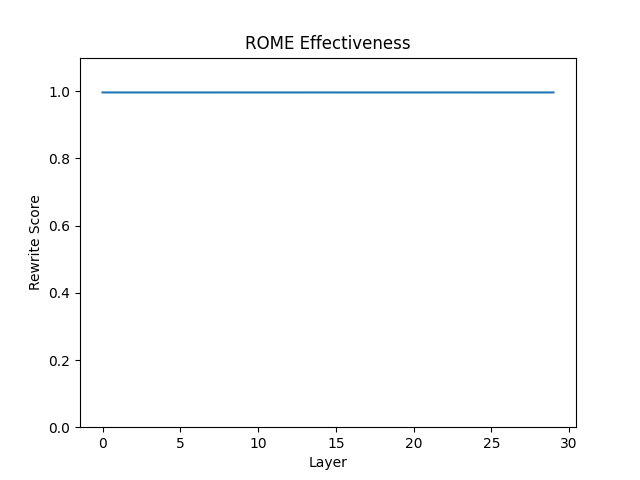
\includegraphics[width=0.5\textwidth]{figures/ROME_rewrite.png}
  \caption{ROME edits achieve a rewrite score over 0.96 across all layers as measured by the CounterFact dataset, regardless of the causal tracing results. \cite{hase2023does}}
  \label{fig:rome_rewrites}
\end{figure}

\section{Extending Causal Tracing: Interchange Interventions}
Despite this setback, I still extended causal tracing to support interchange interventions. 

% \begin{algorithm}[H]\label{alg:causal_tracing}
%   \caption{Causal Tracing Algorithm}
%   \begin{algorithmic}[1]
%   \State \textbf{Clean Run:} Save activations for factual prompt \( x \) as \( \{h_i^l\} \)
%   \State \textbf{Corrupt Run:} Apply noise to subject entity tokens in \( x \), save activations \( \{h_i^{l*}\} \)
%   \State \textbf{Restore at Token \( t \), Layer \( l \):} In corrupted run, replace activation at \( (t, l) \) with clean state \( h_t^l \)
%   \State \textbf{Check Output:} Ensure the output is the same as the clean run
%   \end{algorithmic}
% \end{algorithm}

% \begin{algorithm}[H]\label{alg:interchange_interventions}
%   \caption{Interchange Interventions Algorithm}
%   \begin{algorithmic}[1]
%   \State \textbf{Clean Run:} Save activations for factual prompt \( x \) as \( \{h_i^l\} \)
%   \State \textbf{Alternate Run:} Use source input \( x' \), save activations \( \{h_i^{l'}\} \)
%   \State \textbf{Intervene on Clean Run:} For each layer \( l \) and token \( t \), patch clean run activations \( h_t^l \) with activations from alternate run \( h_t^{l'} \)
%   \State \textbf{Evaluate Output:} Compare the output of the intervened model with the clean run to assess the effect of the intervention
%   \end{algorithmic}
% \end{algorithm}

\begin{figure}[H]
  \centering
  \begin{minipage}{0.48\textwidth}
      \begin{algorithm}[H]
          \caption{Causal Tracing}
          \begin{algorithmic}[1]
          \State \textbf{Clean Run:} Save \( \{h_i^l\} \) for prompt \( x \)
          \State \textbf{Corrupt Run:} Apply noise to \( x \), save \( \{h_i^{l*}\} \)
          \State \textbf{Restore:} In corrupt run, replace \( (t, l) \) with \( h_t^l \)
          \State \textbf{Check Output:} Output of intervened run should match clean run
          \end{algorithmic}
          \label{alg:causal_tracing}
      \end{algorithm}
  \end{minipage}\hfill
  \begin{minipage}{0.48\textwidth}
      \begin{algorithm}[H]
          \caption{Interchange Interventions}
          \begin{algorithmic}[1]
          \State \textbf{Clean Run:} Save \( \{h_i^l\} \) for \( x \)
          \State \textbf{Alternate Run:} Use \( x' \), save \( \{h_i^{l'}\} \)
          \State \textbf{Intervene:} Patch \( h_t^l \) with \( h_t^{l'} \)
          \State \textbf{Evaluate:} Output of intervened run should match target output
          \end{algorithmic}
          \label{alg:interchange_interventions}
      \end{algorithm}
  \end{minipage}
\end{figure}


After implementing this extension, I evaluated it using examples from the CounterFact dataset. In order to do this, I used `attribute prompts' as my source prompts, which generate the desired output:
  
\begin{example}\label{ex:Danielle}
  Consider the following interchange intervention:
  \begin{itemize}
      \item \textbf{Prompt:} ``The mother tongue of Danielle Darrieux is ''
      \item \textbf{Correct Output:} ``French''
      \item \textbf{Attribute Prompt for Interchange Intervention:} ``J.\,R.\,R. Tolkien is a native speaker of ''
      \item \textbf{Desired Output after Intervention:} ``English''
  \end{itemize}
  The intervention should replace the activations at token $t$ and layer $l$ with the activations of the source prompt, and then check if the output is ``English''. However, the results in Figure 2 (left) show that the intervention actually makes the target tokens even less likely than without an edit!
  \end{example}

  \begin{figure}[h]
    \centering
    \begin{minipage}{0.43\textwidth}
        \centering
        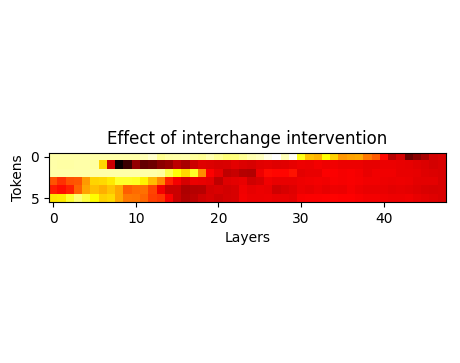
\includegraphics[width=\textwidth]{figures/countereffective_table_0.png}
    \end{minipage}\hfill
    \begin{minipage}{0.57\textwidth}
        \centering
        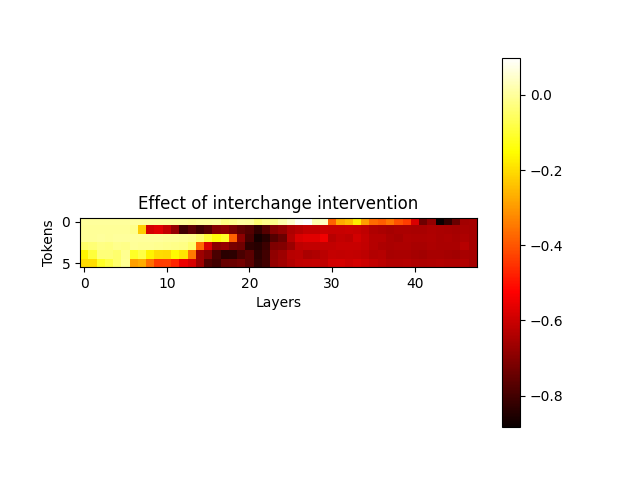
\includegraphics[width=\textwidth]{figures/table_0.png}
    \end{minipage}
    \caption{Effect of interchange intervention for Example \ref{ex:Danielle}. For some reason, the effect is negative: the intervention makes the target tokens even less likely than without an edit! At least prompts which are closer to the target concept (left) perform better than prompts farther away (right). Notably, there is still an early site where the effects manifest, as with causal tracing.}
\end{figure}


%   \begin{figure}[h]
%   \centering
%   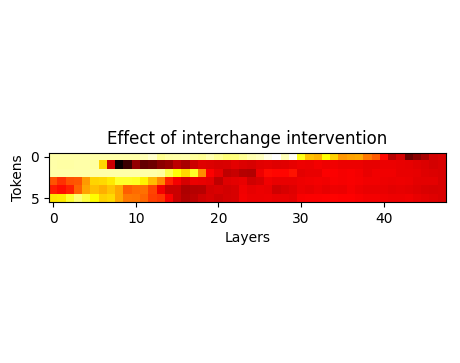
\includegraphics[width=1.0\textwidth]{figures/countereffective_table_0.png}
%   \caption{Effect of interchange intervention for Example \ref{ex:Danielle}.For some reason, the effect is negative: the intervention makes the target tokens even less likely than without an edit! Notably, there is still an early site where the effects manifest, as with causal tracing.}
%   \label{fig:attribute}
% \end{figure}

As a sanity check, I also evaluated the interchange intervention using `neighborhood prompts' as my source prompts, which generate the original unchanged output. For instance, see Example \ref{ex:neighborhood}.

\begin{example}\label{ex:neighborhood}
  Consider the following interchange intervention:
  \begin{itemize}
      \item \textbf{Prompt:} ``The mother tongue of Danielle Darrieux is ''
      \item \textbf{Correct Output:} ``French''
      \item \textbf{Neighborhood Prompt for Interchange Intervention:} ``The mother tongue of Léon Blum is''
      \item \textbf{Desired Output after Intervention:} ``English'' (But the output should remain ``French'')
  \end{itemize}
  The results are shown in figure 2 (right). The intervention is still failing to achieve the desired output, but at least it makes the desired output \emph{less} likely than with the attribute prompt, as expected.
  \end{example}

% \begin{figure}[h]
%   \centering
%   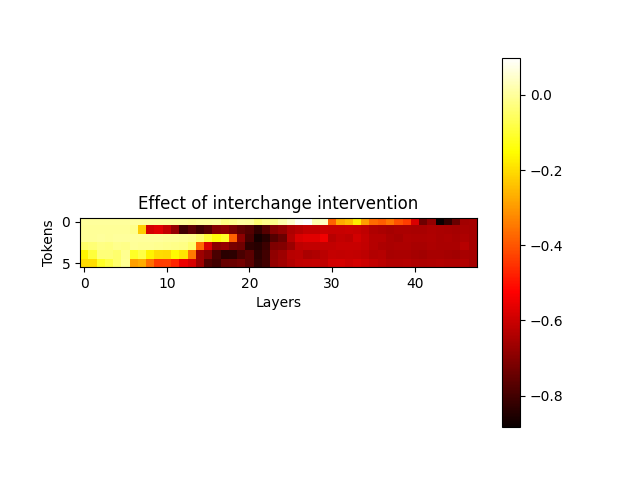
\includegraphics[width=1.0\textwidth]{figures/table_0.png}
%   \caption{.}
%   \label{fig:neighborhood}
% \end{figure}

Overall, I'm unsure if interchange interventions as currently framed are an improvement over causal tracing. However, I suspect this may be a limitation of the implementation: in the original interchange interventions paper \cite{geiger2023finding}, the authors only apply the intervention to a subspace of the activations, \emph{not} the entire activation as in causal tracing. I'll continue to investigate this in my own research.

\section{Conclusion}

In conclusion, I have extended causal tracing to support interchange interventions, and have evaluated it using examples from the CounterFact dataset. The results are mixed: while the intervention is failing to achieve the desired output, it is at least doing worse on source prompts which are farther removed from the target token, as expected. 

%\newpage
\printbibliography

\newpage
\appendix

% \title{Appendix}
% \date{\vspace{-5ex}}
% \maketitle

% \section{Proofs}
% Recall that \cref{thm:mooncracker} is provided to illustrate the use of restatable.
% \mooncracker* 
% \begin{proof}
%   This is straightforward from well-known results of Wallace and Gromit. \PROBLEM{missing citation}
% \end{proof}

\end{document}
